\documentclass{beamer}
\usepackage{multicol}
\usepackage{natbib} 
\usepackage{multirow}
\def\newblock{\hskip .11em plus .33em minus .07em}
\newcommand\independent{\protect\mathpalette{\protect\independenT}{\perp}} 
\def\independenT#1#2{\mathrel{\rlap{$#1#2$}\mkern2mu{#1#2}}} 
%\usepackage{beamerthemeBerkeley}
% Use either the one above or the one below
\usetheme{Pittsburgh}

\title{Instrumental Variables}
%\author{	F. Daniel Hidalgo\\ }
%\date{\today}

\begin{document}

\frame{\titlepage}

%\section[Outline]{}
%\frame{\tableofcontents}

\begin{frame}
  \frametitle{Direct and Indirect Colonial Rule in India}
  \begin{figure}[t]
    \centering
      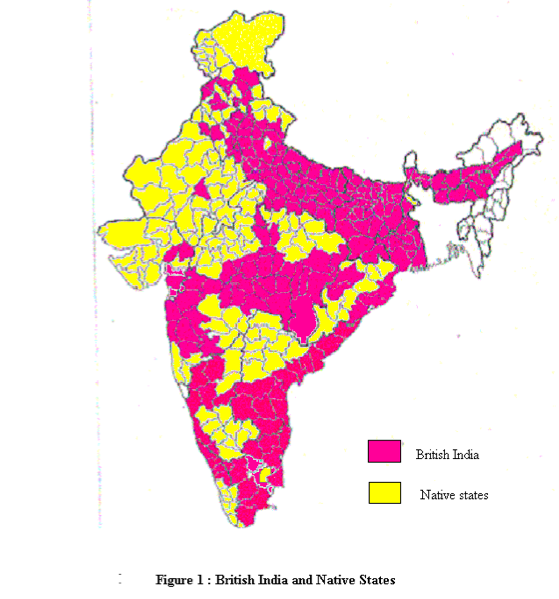
\includegraphics[scale=.35]{indiamap}
 \end{figure}
\end{frame}

\begin{frame}
  \frametitle{Colonial Rule as a "Treatment"}
  \begin{itemize}
  \item 415 districts, some of which were formerly part of British
    India.
  \item Indicate treatment by a dummy variable: 
    $D_i=1$ if the district remained under direct colonial control
    until independence or $D_i=0$ if it remained part of a ``native''
    state.
  \item Focus on sample of districts (n=136) which beginning in 1848 were
    parts of native states.
  \item 36 districts (26\%) were eventually \textit{annexed} by the British
    Government. 
  \end{itemize}
\end{frame}

\begin{frame}
  \frametitle{Naive Estimates of the Effect of Colonial Rule}
  \begin{itemize}
  \item DV is a measure of public good provision in the district (from
    the 1980/1990 censuses).
  \item Ideally, we want to know:
$$\mathbb{E}[\delta] =
\mathbb{E}[Y(1)-Y(0)]$$
\item We only observe the following:
\begin{eqnarray*}
\mathbb{E}[Y(1)|D=1] - \mathbb{E}[Y(0)|D=0]
\end{eqnarray*}
\item Works under the assumption that districts were annexed ``as-if''
  random.
 \end{itemize}
\end{frame}

 \begin{frame}
   \frametitle{Naive Estimates}
 \begin{figure}[t]
    \centering
      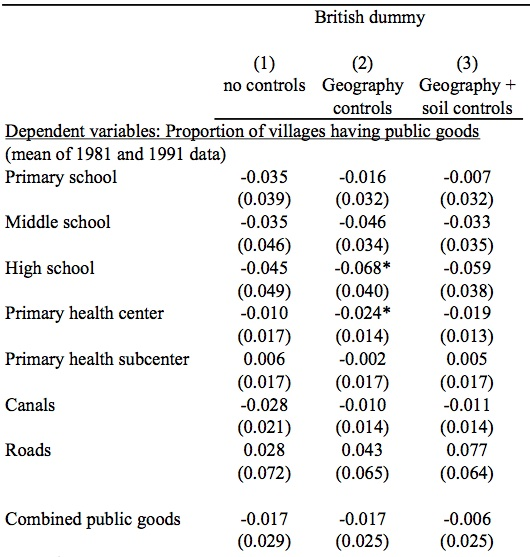
\includegraphics[scale=.8]{naive}
 \end{figure}
 \end{frame}

 \begin{frame}
   \frametitle{The Doctrine of Lapse}
   Lord Dalhousie, Governor-General of India from 1848-1856, enacted a
   new policy regarding annexation:
   \begin{quote}
     I hold that on all occasions where heirs natural shall fail, the territory should be made to lapse and adoption should not be permitted, excepting in those cases in which some strong political reason may render it expedient to depart from this general rule.
   \end{quote}
   \end{frame}


   \begin{frame}
     \frametitle{The Doctrine of Lapse}
     \begin{itemize}
     \item Now we have a new variable,   $Z_i=1$ if the district's
       ruler without an heir or  $Z_i=0$ with an heir. Note that $Z_i \neq D_i
       \forall i$, so the Doctrine of Lapse is not always followed. 
     \item Iyer claims that while the assumption that
       $(Y(0),Y(1))\independent D$ is not plausible, the assumption
       $(Y(0),Y(1))\independent Z$ is plausible.
     \item Under her assumptions,
\begin{eqnarray*}
\hat \delta_Z & =&\mathbb{E}[Y(1)|Z=1] - \mathbb{E}[Y(0)|Z=0]  \\
&=&\mathbb{E}[Y(1)] - \mathbb{E}[Y(0)] 
\end{eqnarray*}
     \end{itemize}
Do we care about this estimand? 
\end{frame}

\begin{frame}
  \frametitle{The Doctrine of Lapse as an Instrument}
  \begin{itemize}
  \item Let's rewrite $D_i$ as $D_i(Z_i)$ to reflect the fact that
    whether or not a district is annexed can depend on whether or not
    the ruler dies without an heir.
  \item Similarly, we can rewrite the potential outcomes as
    $Y_i(D_i,Z_i)$.
  \item The causal effect of $Z$ on colonial rule for an individual
    district can be written as $D_i(1)-D_i(0)$. The causal effect of
    $Z$ on socioeconomic outcomes can be written as
    $Y_i(1,D(1)-Y_i(0,D(0))$, which is the ``intent to treat''
    effect. 
  \end{itemize}
Now we need assumptions:
  \begin{enumerate}
  \item SUTVA
  \item (``as if'') Random Assignment of $Z_i$.
  \item Exclusion restriction: $Y_i(1, D_i)=Y_i(0,D_i)$.
  \item Non-zero average causal effect of $Z$ on $D$.
  \item Montonicity: $D_i(1) \geq D_1(0)$ for all $i$.
  \end{enumerate}
\end{frame}

\begin{frame}
  \frametitle{The Exclusion Restriction}
  \begin{figure}[t]
    \centering
      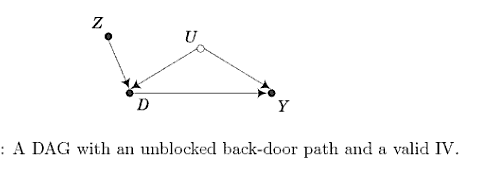
\includegraphics[scale=.7]{DAG}
 \end{figure}
\end{frame}

\begin{frame}
  \frametitle{The First Stage}
  \begin{figure}[t]
    \centering
      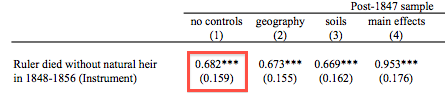
\includegraphics[scale=.7]{first_stage}
 \end{figure}
\end{frame}

\begin{frame}
  \frametitle{Deriving the IV Estimator}
  \begin{itemize}
  \item First, let's redefine the individual causal effect using the
    exclusion restriction:
\begin{eqnarray*}
Y_i(1,D(1)-Y_i(0,D(0))& =& Y_i(D(1)-Y_i(D(0))  \\
&=& (Y_i(1)-Y_i(0))\cdot (D_i(1)-D_i(0))
\end{eqnarray*}
\item Now we need to focus on average effects. We've assumed that
  $\mathbb{E}[D_i(1)-D_i(0)] \neq 0$. So we can decompose the average
  causal effect as:
  \begin{eqnarray*}
   & \mathbb{E}[Y_i(D_i(1))-Y_i(D_i(0))] \\
 = & \mathbb{E}[(Y_i(1)-Y_i(0))|(D_i(1)-D_i(0)=1)] \cdot
 P[D_i(1)-D_i(0)=1] \\
&-\mathbb{E}[(Y_i(1)-Y_i(0))|(D_i(1)-D_i(0)=-1)] \\ 
&\cdot
 P[D_i(1)-D_i(0)=-1]
  \end{eqnarray*}
  \end{itemize}
\end{frame}
\begin{frame}
  \frametitle{Deriving the IV Estimator}
  \begin{itemize}
  \item Ok, now we have 5 unknowns, of which we can calculate only
    1 of them from the data. To get rid of some unknowns, we invoke the monotinicity
    assumption, which leaves us with:
  \begin{eqnarray*}
   &\mathbb{E}[Y_i(D_i(1))-Y_i(D_i(0))]  \\
 = & \mathbb{E}[(Y_i(1)-Y_i(0))|(D_i(1)-D_i(0)=1)] \cdot
 P[D_i(1)-D_i(0)=1]
  \end{eqnarray*}
\item Now we have three unknowns, 2 which of can be estimated with the
  data. Under the monotonicity assumption  $P[D_i(1)-D_i(0)=1] =
  \mathbb{E}[D_i(1)-D_i(0)] $, which is simply the the effect of the
  instrument on treatment assignment status.
\item Solving for $\mathbb{E}[(Y_i(1)-Y_i(0))|(D_i(1)-D_i(0)=1)]$, we
  get the following expression for our IV estimator: $$\frac{\mathbb{E}[Y_i(D_i(1))-Y_i(D_i(0))] }{\mathbb{E}[D_i(1)-D_i(0)] }$$
  \end{itemize}
\end{frame}
\begin{frame}
  \frametitle{What is the IV estimand?}
  \begin{table}[h]
    \centering
    \begin{tabular}{c c c c}
& & \multicolumn{2}{c}{$D_i(0)$} \\ \hline
& & 0 & 1 \\ \hline
\multirow{2}{*}{$D_i(1)$}&0 & Never-taker & Defier\\
&1 & Complier & Always-taker \\ \hline
      
    \end{tabular}
    \caption{Causal Types}
  \end{table}
  \begin{itemize}
  \item $\mathbb{E}[(Y_i(1)-Y_i(0))|(D_i(1)-D_i(0)=1)]$ is the causal
    effect of the treatment on compliers, a kind of LATE. 
  \item In our example, it's the causal effect of British direct rule
    on those districts induced by the Doctrine of Lapse to lose their
    independent status.  
  \end{itemize}
\end{frame}

\begin{frame}
  \frametitle{IV Results}
  \begin{figure}[t]
    \centering
      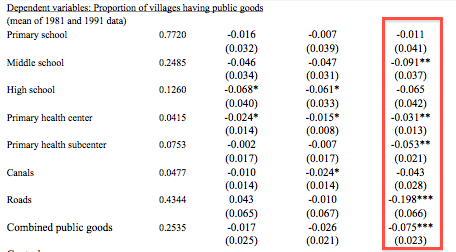
\includegraphics[scale=.7]{ivresults}
 \end{figure}
\end{frame}



\end{document}
